% CS631 Advanced Programming in the UNIX Environment
% Author: Jan Schaumann <jschauma@netmeister.org>
% $Id: slides.tex,v 1.5 2004/08/04 03:03:44 jschauma Exp $

\documentclass[xga]{xdvislides}
\usepackage[landscape]{geometry}
\usepackage{graphics}
\usepackage{graphicx}
\usepackage{colordvi}

\begin{document}
\setfontphv

%%% Headers and footers
\lhead{\slidetitle}
\chead{CS631 - Advanced Programming in the UNIX Environment}
\rhead{Slide \thepage}
\lfoot{\Gray{Lecture 09: Interprocess Communication II}}
\cfoot{\relax}
\rfoot{\Gray{\today}}

\vspace*{\fill}
\begin{center}
	\Hugesize
		CS631 - Advanced Programming in the UNIX Environment\\
		%\vspace{.1in}\includegraphics[scale=0.5]{pics/j1.eps} \\
		Interprocess Communication II\\
	\hspace*{5mm}\blueline\\ [1em]

	\Normalsize
		Department of Computer Science\\
		Stevens Institute of Technology\\
		Jan Schaumann\\
		\verb+jschauma@cs.stevens.edu+\\
		\verb+https://stevens.netmeister.org/631/+
\end{center}
\vspace*{\fill}


\subsection{Pipes: {\tt pipe(2)}}
\small
\setlength{\unitlength}{1mm}
\begin{center}
	\begin{picture}(150,22)
		\thinlines
		\put(0,0){\framebox(130,22){}}
		\put(10,17){{\tt \#include <unistd.h>}}
		\put(10,10){{\tt int pipe(int {\em filedes[2]});}}
		\put(80,3){Returns: 0 if OK, -1 otherwise}
	\end{picture}
\end{center}
\Normalsize
\begin{itemize}
	\item oldest and most common form of UNIX IPC
	\item half-duplex (on some versions full-duplex)
	\item can only be used between processes that have a common ancestor
	\item can have multiple readers/writers ({\tt PIPE\_BUF} bytes are
		guaranteed to not be interleaved)
\end{itemize}
\vspace{.5in}

Behavior after closing one end:
\begin{itemize}
	\item {\tt read(2)} from a pipe whose write end has been closed returns 0
		after all data has been read
	\item {\tt write(2)} to a pipe whose read end has been closed generates
		{\tt SIGPIPE} signal.  If caught or ignored, {\tt write(2)} returns an
		error and sets {\tt errno} to {\tt EPIPE}.
\end{itemize}

\subsection{Pipes: {\tt pipe(2)}}
\begin{center}
	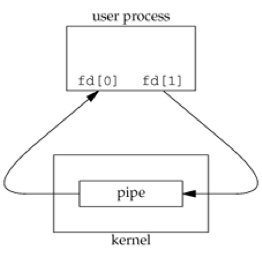
\includegraphics[angle=-90,scale=0.8]{pics/pipe1.eps}
\end{center}

\subsection{Pipes: {\tt pipe(2)}}
\begin{center}
	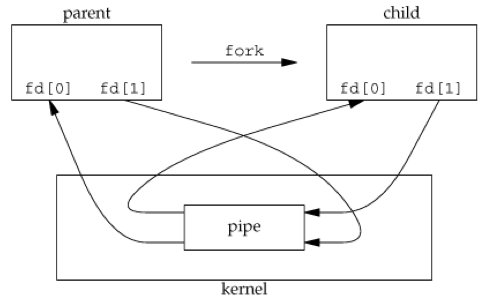
\includegraphics[angle=-90,scale=0.8]{pics/pipe2.eps}
\end{center}

\subsection{Pipes: {\tt pipe(2)}}
\begin{center}
	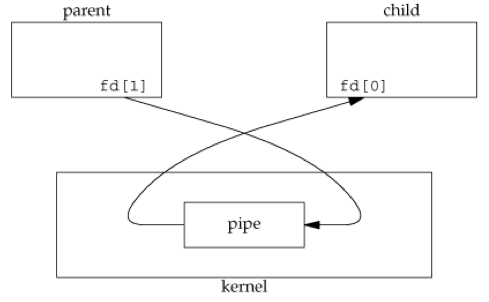
\includegraphics[angle=-90,scale=0.8]{pics/pipe3.eps}
\end{center}

\subsection{Sockets: {\tt socketpair(2)}}
\small
\setlength{\unitlength}{1mm}
\begin{center}
	\begin{picture}(150,22)
		\thinlines
		\put(0,0){\framebox(130,22){}}
		\put(10,17){{\tt \#include <sys/socket.h>}}
		\put(10,10){{\tt int socketpair(int {\em domain}, int {\em type}, int {\em protocol}, int *{\em sv});}}
	\end{picture}
\end{center}
\Normalsize

The {\tt socketpair(2)} call creates an unnamed pair of connected sockets in
the specified domain {\tt domain}, of the specified {\em type}, and using the
optionally specified {\em protocol}.
\\

The descriptors used in referencing the new sockets are returned in {\em
sv[0]} and {\em sv[1]}.  The two sockets are indistinguishable.
\\

{\tt This call is currently implemented only for the UNIX domain.}


\subsection{Sockets: {\tt socketpair(2)}}
\begin{center}
	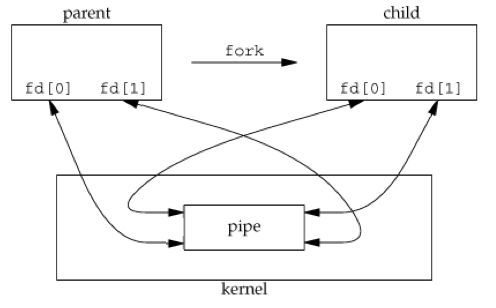
\includegraphics[angle=-90,scale=0.8]{pics/socketpair1.eps}
\end{center}

\subsection{Sockets: {\tt socketpair(2)}}
\begin{center}
	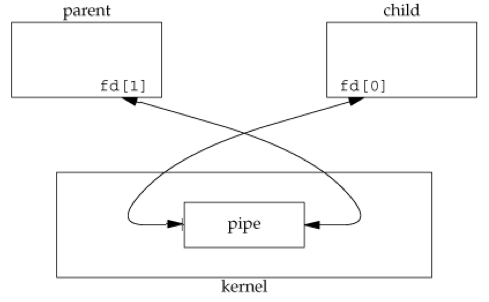
\includegraphics[angle=-90,scale=0.8]{pics/socketpair2.eps}
\end{center}

\subsection{Sockets: {\tt socketpair(2)}}
\begin{verbatim}
$ cc -Wall socketpair.c
$ ./a.out
78482 --> sending: In Xanadu, did Kublai Khan . . .
78483 --> sending: A stately pleasure dome decree . . .
78483 --> reading: In Xanadu, did Kublai Khan . . .
78482 --> reading: A stately pleasure dome decree . . .
$
\end{verbatim}
\vfill
%\hfill \includegraphics[angle=-90,scale=0.9]{pics/j6.eps}


\subsection{Sockets: {\tt socket(2)}}
\small
\setlength{\unitlength}{1mm}
\begin{center}
	\begin{picture}(150,22)
		\thinlines
		\put(0,0){\framebox(130,22){}}
		\put(10,17){{\tt \#include <sys/socket.h>}}
		\put(10,10){{\tt int socket(int {\em domain}, int {\em type}, int {\em protocol});}}
	\end{picture}
\end{center}
\Normalsize
Some of the currently supported domains are:
\\

\small
\begin{tabular}{| l | l |}
	\hline
	{\bf Domain} & {\bf Description} \\
	\hline
	{\tt PF\_LOCAL} 	& 	local (previously UNIX) domain protocols \\
	{\tt PF\_INET}		&	ARPA Internet protocols \\
	{\tt PF\_INET6}		&	ARPA IPv6 (Internet Protocol version 6) protocols \\
	{\tt PF\_ARP}		&	RFC 826 Ethernet Address Resolution Protocol\\
	{\tt ...}		&	...\\
	\hline
\end{tabular}
\Normalsize
\vspace{.5in}

Some of the currently defined types are:
\\

\small
\begin{tabular}{| l | l |}
	\hline
	{\bf Type}		&	{\bf Description} \\
	\hline
	{\tt SOCK\_STREAM}	&	sequenced, reliable, two-way connection based byte streams \\
	{\tt SOCK\_DGRAM}	&	connectionless, unreliable messages of a fixed (typically small)
							maximum length \\
	{\tt SOCK\_RAW}		&	access to internal network protocols and interfaces \\
	{\tt ...}		&	... \\
	\hline
\end{tabular}
\Normalsize

\subsection{Sockets: Datagrams in the UNIX/LOCAL domain}
\begin{verbatim}
1$ cc -Wall udgramsend.c -o send
1$ cc -Wall udgramread.c -o read
1$ ./read
socket --> socket

2$ ls -l socket
srwxr-xr-x  1 jans  users   0 Oct 31 19:17 socket
2$ ./send socket
2$

--> The sea is calm tonight, the tide is full . . .
1$
\end{verbatim}
\vfill
%\hfill \includegraphics[scale=0.9]{pics/j7.eps}


\subsection{Sockets: Datagrams in the UNIX/LOCAL domain}
\begin{itemize}
	\item create socket using {\tt socket(2)}
	\item attach to a socket using {\tt bind(2)}
	\item binding a name in the UNIX domain creates a socket in the file system
	\item both processes need to agree on the name to use
	\item these files are only used for rendezvous, not for message delivery
		once a connection has been established
	\item sockets must be removed using {\tt unlink(2)}
\end{itemize}

\subsection{Sockets: Datagrams in the Internet Domain}
\begin{verbatim}
1$ cc -Wall dgramsend.c -o send
1$ cc -Wall dgramread.c -o read
1$ ./read
Socket has port #64293

2$ netstat -na | grep 64293
udp4       0      0  *.64293                *.*
2$ ./send localhost 64293
2$

--> The sea is calm tonight, the tide is full . . .
1$
\end{verbatim}
\vfill
(Compare observed packets via {\tt tcpdump(8)}.)
%\hfill \includegraphics[angle=-90,scale=0.9]{pics/j8.eps}

\subsection{Sockets: Datagrams in the Internet Domain}
\begin{itemize}
	\item Unlike UNIX domain names, Internet socket names are not entered into
		the file system and, therefore, they do not have to be unlinked after the
		socket has been closed.
	\item The local machine address for a socket can be any valid network address
		of the machine, if it has more than one, or it can be the wildcard value
		{\tt INADDR\_ANY}.
	\item ``well-known'' ports (range 1 - 1023) only available to super-user
	\item request any port by calling {\tt bind(2)} with a port number of 0
	\item determine used port number (or other information) using {\tt
		getsockname(2)}
	\item convert between network byteorder and host byteorder using {\tt
		htons(3)} and {\tt ntohs(3)} (which may be noops)
	\item you can (try to) send packets without anything listening (connectionless, unreliable)
\end{itemize}

\subsection{Sockets: Connections using stream sockets}
\begin{verbatim}
1$ cc -Wall streamread.c -o read
1$ cc -Wall streamwrite.c -o write
1$ ./read
Socket has port #65398

2$ ./write localhost 65398
2$ ./write localhost 65398
--> Half a league, half a league . . .
Ending connection
--> Half a league, half a league . . .
Ending connection

2$ nc localhost 65398
moo
2$
\end{verbatim}
\vfill
%\hfill \includegraphics[angle=-90,scale=0.9]{pics/j9.eps}

\subsection{Sockets: Connections using stream sockets}
\begin{itemize}
	\item connections are asymmetrical:  one process requests a connection,
		the other process accepts the request
	\item one socket is created for each accepted request
	\item mark socket as willing to accept connections using {\tt listen(2)}
	\item pending connections are then {\tt accept(2)}ed
	\item {\tt accept(2)} will block if no connections are available
\end{itemize}

\subsection{I/O Multiplexing}
Standard I/O loop:
\begin{verbatim}
while ((n = read(fd1, buf, BUFFSIZE)) > 0) {
        if (write(fd2, buf, n) != n) {
                fprintf(stderr, "write error\n");
                exit(1);
         }
}
\end{verbatim}

Suppose you want to read from multiple file descriptors - now what?



\subsection{I/O Multiplexing}
When handling I/O on multiple file descriptors, we have the following
options:

\begin{itemize}
	\item blocking mode: open one fd, block, wait (possibly forever),
		then test the next fd
	\item fork and use one process for each, communicate using signals
		or other IPC
	\item non-blocking mode: open one fd, immediately get results,
		open next fd, immediately get results, sleep for some time
	\item asynchronous I/O: get notified by the kernel when either fd
		is ready for I/O
\end{itemize}

\subsection{I/O Multiplexing}
Instead of blocking forever (undesirable), using {\em non-blocking} mode
(busy-polling is inefficient) or using {\em asynchronous I/O} (somewhat
limited), we can:
\begin{itemize}
	\item build a set of file descriptors we're interested in
	\item call a function that will return if any of the file
		descriptors are ready for I/O (or a timeout has elapsed)
\end{itemize}

\subsection{I/O Multiplexing}
\small
\setlength{\unitlength}{1mm}
\begin{center}
	\begin{picture}(180,40)
		\thinlines
		\put(0,0){\framebox(160,40){}}
		\put(10,35){{\tt \#include <sys/types.h>}}
		\put(10,30){{\tt \#include <sys/time.h>}}
		\put(10,25){{\tt \#include <unistd.h>}}
		\put(10,18){{\tt int select(int {\em maxfdp1}, fd\_set *{\em readfds}, fd\_set *{\em writefds}}}
		\put(40,13){{\tt fd\_set *{\em exceptfds}, struct timeval *{\em tvptr});}}
		\put(60,5){Returns: count of ready descriptors, 0 on timeout, -1 otherwise}
	\end{picture}
\end{center}
\Normalsize
Arguments passed:
\begin{itemize}
	\item which descriptors we're interested in
	\item what conditions we're interested in
	\item how long we want to wait
		\begin{itemize}
			\item {\tt tvptr == NULL} means wait forever
			\item {\tt tvptr->tv\_sec == tvptr->tv\_usec == 0} means don't wait at all
			\item wait for specified amount of time
		\end{itemize}
\end{itemize}
\vspace{.25in}
{\tt select(2)} tells us both the total count of descriptors that are
ready as well as which ones are ready.


\subsection{I/O Multiplexing}
\begin{itemize}
	\item filedescriptor sets are manipulated using the {\tt FD\_*} functions/macros
	\item read/write sets indicate readiness for read/write; {\em except} indicates an exception condition (for example OOB data, certain terminal events)
	\item EOF means ready for read - {\tt read(2)} will just return 0 (as usual)
	\item {\tt pselect(2)} provides finer-grained timeout control;
allows you to specify a signal mask (original signal mask is restored
upon return)
	\item {\tt poll(2)} provides a conceptually similar interface
\end{itemize}
\vspace{.5in}
See also: \verb+https://daniel.haxx.se/docs/poll-vs-select.html+

\subsection{Sockets: Connections using stream sockets}
\begin{verbatim}
1$ cc -Wall strchkread.c -o read
1$ ./read
Socket has port #65398
Do something else
Do something else
2$ ./write localhost 65398
2$ ./write localhost 65398
‐-> Half a league, half a league . . .
Ending connection
Do something else
--> Half a league, half a league . . .
Ending connection
^C
1$
\end{verbatim}
\vfill
%\hfill \includegraphics[angle=-90,scale=0.6]{pics/j10.eps}


\subsection{Sockets: Other Useful Functions}

I/O on sockets is done on descriptors, just like regular I/O, ie the typical
{\tt read(2)} and {\tt write(2)} calls will work.  In order to specify certain
flags, some other functions can be used:

\begin{itemize}
	\item {\tt send(2)}, {\tt sendto(2)} and {\tt sendmsg(2)}
	\item {\tt recv(2)}, {\tt recvfrom(2)} and {\tt recvmsg(2)}
\end{itemize}
To manipulate the options associated with a socket, use {\tt setsockopt(2)}:
\small
\begin{tabular}{| l | l |}
	\hline
	{\bf Option}		&	{\bf Description} \\
	\hline
	{\tt SO\_DEBUG}		&	enables recording of debugging information \\
	{\tt SO\_REUSEADDR}	&	enables local address reuse \\
	{\tt SO\_REUSEPORT}	&	enables duplicate address and port bindings \\
	{\tt SO\_KEEPALIVE}	&	enables keep connections alive\\
	{\tt SO\_DONTROUTE}	&	enables routing bypass for outgoing messages\\
	{\tt SO\_LINGER}	&	linger on close if data present\\
	{\tt SO\_BROADCAST}	&	enables permission to transmit broadcast messages\\
	{\tt SO\_OOBINLINE}	&	enables reception of out-of-band data in band\\
	{\tt SO\_SNDBUF}	&	set buffer size for output\\
	{\tt SO\_RCVBUF}	&	set buffer size for input\\
	{\tt SO\_SNDLOWAT}	&	set minimum count for output\\
	{\tt SO\_RCVLOWAT}	&	set minimum count for input\\
	{\tt SO\_SNDTIMEO}	&	set timeout value for output\\
	{\tt SO\_RCVTIMEO}	&	set timeout value for input\\
	{\tt SO\_TIMESTAMP}	&	enables reception of a timestamp with datagrams\\
	{\tt SO\_TYPE}		&	get the type of the socket (get only)\\
	{\tt SO\_ERROR}		&	get and clear error on the socket (get only)\\
	\hline
\end{tabular}
\Normalsize

\subsection{Final Project}

Write a simple web server. \\
\verb+https://stevens.netmeister.org/631/f18-final-project.html+

\subsection{More Information}
Reading:
\begin{itemize}
	\item \verb+https://stevens.netmeister.org/ipc.pdf+
	\item \verb+https://ops.tips/blog/how-linux-creates-sockets/+
	\item \verb+https://ops.tips/blog/how-linux-tcp-introspection/+
	\item \verb+https://beej.us/guide/bgipc/html/single/bgipc.html+
\end{itemize}
\vspace{.5in}

%\begin{center}
%\includegraphics[angle=-90,scale=0.75]{pics/nbc.eps}
%\end{center}
%\vspace{\fill}
%\small
%\hfill ...And they call him, Sandy... Clawssss...!

Exercises:
\begin{itemize}
	\item Revisit HW2; try to implement it using a
		{\tt socketpair(2)}
	\item What happens if you change the {\tt
domain}, {\tt type}, and {\tt protocol} arguments to
{\tt socketpair(2)}?
	\item Even though communications via {\tt
localhost} work just fine, make sure to verify network
communications across the internet.
\end{itemize}


\end{document}
